\documentclass[cs4size,a4paper,10pt]{ctexart}   

\linespread{1.5}
\usepackage{geometry}%用于设置上下左右页边距
	\geometry{left=2.5cm,right=2.5cm,top=3.2cm,bottom=2.7cm}
\usepackage{xeCJK,amsmath,paralist,enumerate,booktabs,multirow,graphicx,subfig,setspace,listings,lastpage,hyperref}
\usepackage{amsthm, amssymb, bm, color, framed, graphicx, hyperref, mathrsfs}
\usepackage{mathrsfs}  
	\setlength{\parindent}{2em}
	\lstset{language=Matlab}%
\usepackage{fancyhdr}
\usepackage{graphicx}
\usepackage{subfloat}
\usepackage{listings}
\usepackage{xcolor}
\usepackage{float}
\usepackage{paralist}
\usepackage{setspace}
\usepackage{titlesec}
\usepackage{enumitem}
\usepackage{hyperref}
\usepackage{multirow}
\usepackage{threeparttable}
\usepackage{autobreak}
\usepackage{multicol}
\usepackage{subfig}
\usepackage{unicode-math}
\usepackage{ltxtable, filecontents}
\usepackage{array}

\hypersetup{
	colorlinks=true,
	linkcolor=black,
	urlcolor=black
}

\setenumerate{partopsep=0pt,topsep=0pt}
\setitemize{itemsep=0pt,partopsep=0pt,topsep=0pt}

\titlespacing*{\section}{0pt}{3pt}{3pt}
\titlespacing*{\subsection}{0pt}{2pt}{2pt}
\titlespacing*{\subsubsection}{0pt}{1pt}{1pt}
\titlespacing*{\paragraph}{0pt}{0pt}{0pt}

\ctexset{secnumdepth=4,tocdepth=4}
\setlength{\parindent}{0pt}
\setstretch{1.2}


\setCJKmainfont[BoldFont={FZHei-B01},ItalicFont={FZKai-Z03}]{FZShuSong-Z01} 
\setCJKsansfont[BoldFont={FZHei-B01}]{FZKai-Z03} 
\setCJKmonofont[BoldFont={FZHei-B01}]{FZFangSong-Z02}
\setCJKfamilyfont{zhsong}{FZShuSong-Z01} 
\setCJKfamilyfont{zhhei}{FZHei-B01} 
\setCJKfamilyfont{zhkai}[BoldFont={FZHei-B01}]{FZKai-Z03} 
\setCJKfamilyfont{zhfs}[BoldFont={FZHei-B01}]{FZFangSong-Z02} 
\renewcommand*{\songti}{\CJKfamily{zhsong}} 
\renewcommand*{\heiti}{\CJKfamily{zhhei}} 
\renewcommand*{\kaishu}{\CJKfamily{zhkai}} 
\renewcommand*{\fangsong}{\CJKfamily{zhfs}}


\definecolor{mKeyword}{RGB}{0,0,255}          % bule
\definecolor{mString}{RGB}{160,32,240}        % purple
\definecolor{mComment}{RGB}{34,139,34}        % green
\definecolor{mNumber}{RGB}{128,128,128} 

\lstdefinestyle {njulisting} {
	basewidth = 0.5 em,
	lineskip = 3 pt,
	basicstyle = \small\ttfamily,
	% keywordstyle = \bfseries,
	commentstyle = \itshape\color{gray}, 
	basicstyle=\small\ttfamily,
	keywordstyle={\color{black}},     % sets color for keywords
	stringstyle={\color{black}},       % sets color for strings
	commentstyle={\color{black}},     % sets color for comments
	numberstyle=\tiny\color{black},
	numbers = left,
	captionpos = t,
	breaklines = true,
	xleftmargin = 1 em,
	xrightmargin = 0 em,
	frame=tlrb,
	tabsize=4,
	aboveskip = 7 pt, %与代码环境上一行的垂直间距
    belowskip = -2 pt %与代码环境下一行的垂直间距
}

\lstset{
style = njulisting, % 调用上述样式 
flexiblecolumns % 允许调整字符宽度
}

\newcommand \sverb {\ \verb}

%================= 基本格式预置 ===========================
\usepackage{fancyhdr}
\pagestyle{fancy}
\lhead{数据管理基础}
\rhead{数据库安全性}
\cfoot{\thepage}
\renewcommand{\headrulewidth}{0.4pt}
\renewcommand{\theenumi}{(\arabic{enumi})}
\CTEXsetup[format={\bfseries\zihao{-3}}]{section}
\CTEXsetup[format={\bfseries\zihao{4}}]{subsection}
\CTEXsetup[format={\bfseries\zihao{-4}}]{subsubsection}


\renewcommand{\contentsname}{目录}  
\begin{document}

	\begin{center}
		{\huge\textbf{第四章\ 数据库安全性}}
	\end{center}
	%---------目录---------% 
	\pagenumbering{Roman}
	\tableofcontents
	\clearpage

 	%---------正文---------% 
	\pagenumbering{arabic}
	\setcounter{page}{1}
	\setlength{\parskip}{0.65em}

	\setlength\abovedisplayskip{5pt}
	\setlength\belowdisplayskip{5pt}

	\section{数据库安全性概述}

\subsection{数据库的不安全因素}
\begin{itemize}
    \item 非授权用户对数据库的恶意存取和破坏
    \begin{itemize}
        \item 一些黑客和犯罪分子在用户存取数据库时猎取用户名和用户口令,然后假冒合法用户偷取、修改甚至破坏用户数据
        \item 数据库管理系统提供的安全措施主要包括用户身份鉴别、存取控制和视图等技术
    \end{itemize}
    \item 数据库中重要或敏感的数据被泄露
    \begin{itemize}
        \item 黑客和敌对分子千方百计盗窃数据库中的重要数据,一些机密信息被暴露
        \item 数据库管理系统提供的主要技术有强制存取控制、数据加密存储和加密传输等
        \item 审计日志分析
    \end{itemize}
    \item 安全环境的脆弱性
    \begin{itemize}
        \item 数据库的安全性与计算机系统的安全性紧密联系
        \item 建立一套可信计算机系统的概念和标准
    \end{itemize}
\end{itemize}

\subsection{安全标准简介}
TCSEC/TDI 安全级别划分
\begin{itemize}
    \item 按系统可靠或可信程度逐渐增高
    \item 各安全级别之间具有一种偏序向下兼容的关系
\end{itemize}

\begin{table}[H]
    \vspace{-0.5em}
    \centering
    \begin{tabular}{|c|c|}
    \hline
    \textbf{安全级别} & \textbf{定义}                               \\ \hline
    A1            & 验证设计(Verified Design)                     \\ \hline
    B3            & 安全域(Security Domains)                     \\ \hline
    B2            & 结构化保护(Structural Protection)              \\ \hline
    B1            & 标记安全保护(Labeled Security Protection)       \\ \hline
    C2            & 受控的存取保护(Controlled Access Protection)     \\ \hline
    C1            & 自主安全保护(Discretionary Security Protection) \\ \hline
    D             & 最小保护(Minimal Protection)                  \\ \hline
    \end{tabular}
    \vspace{-1em}
\end{table}

CC 评估保证级(EAL)划分
\vspace{-0.5em}
\begin{longtable}{|W{c}{1.8cm}|m{8.5cm}<{\centering}|m{3cm}<{\centering}|}
    \hline
    \textbf{评估保证级} & \textbf{定义}                                            & \textbf{TCSEC安全级别(近似相当)} \\ \hline
    EAL1           & 功能测试(functionally tested)                              &                          \\ \hline
    EAL2           & 结构测试(structurally tested)                              & C1                       \\ \hline
    EAL3           & 系统地测试和检查(methodically tested and checked)              & C2                       \\ \hline
    EAL4           & 系统地设计、测试和复查(methodically designed,tested,and reviewed) & B1                       \\ \hline
    EAL5           & 半形式化设计和测试(semiformally designed and tested)            & B2                       \\ \hline
    EAL6           & 半形式化验证的设计和测试(semiformally verified design and tested)  & B3                       \\ \hline
    EAL7           & 形式化验证的设计和测试(formally verified design and tested)       & A1                       \\ \hline
\end{longtable}
\vspace{-1em}

\section{数据库安全性控制}
\begin{figure}[H]
    \vspace{-0.5em}
	\centering
	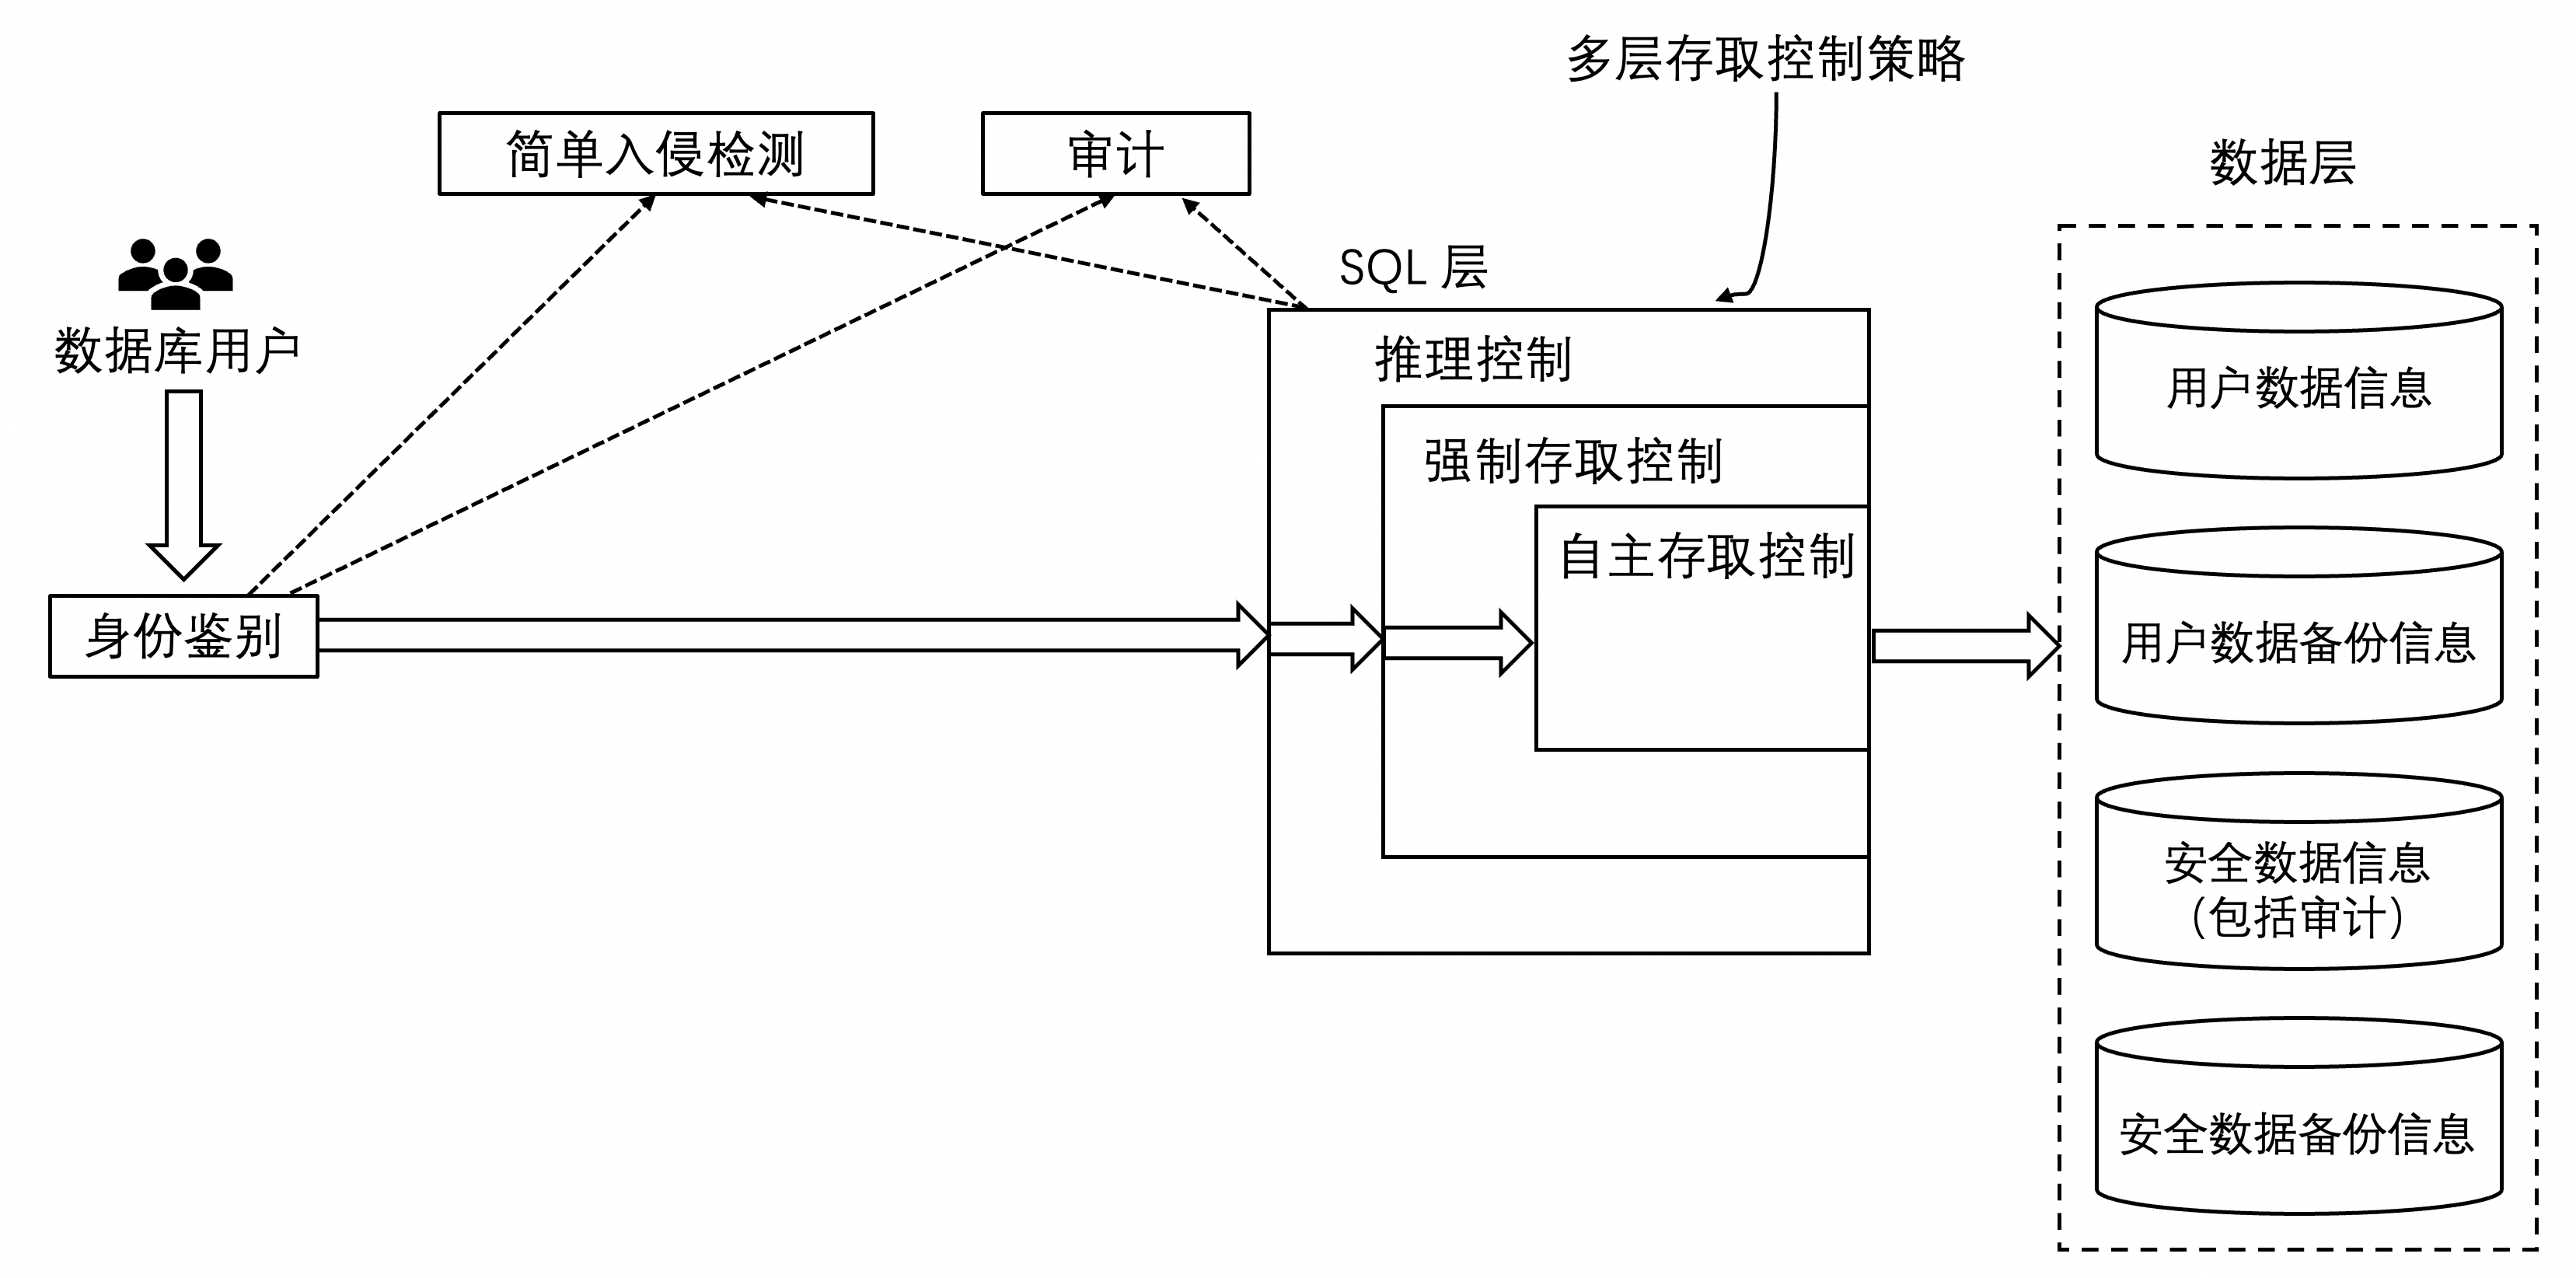
\includegraphics[width=0.85\textwidth]{images/4.2}
    \vspace{-1em}
\end{figure}

\subsection{用户身份鉴别}
\vspace{-0.8em}
\begin{multicols}{4}
    \begin{itemize}
        \item 静态口令鉴别
        \item 动态口令鉴别
        \item 生物特征鉴别
        \item 智能卡鉴别
    \end{itemize}
\end{multicols}
\vspace{-1em}

\subsection{存取控制}
\begin{itemize}
    \item 定义用户权限,并将用户权限登记到数据字典中
    \begin{itemize}
        \item 用户对某一数据对象的操作权力称为权限
        \item DBMS 提供适当的语言来定义用户权限,存放在数据字典中,称做安全规则或授权规则
    \end{itemize}
    \item 合法权限检查 
    \item 用户权限定义和合法权检查机制一起组成了数据库管理系统的存取控制子系统
    \item C2 级的数据库管理系统支持自主存取控制(Discretionary Access Control,DAC),B1 级的数据库管理系统支持强制存取控制(Mandatory Access Control,MAC)
    \begin{itemize}
        \item 在自主存取控制方法中,用户对不同的数据对象有不同的存取权限,不同的用户对同一对象也有不同的权限,而且用户还可将其拥有的存取权限转授给其他用户
        \item 在强制存取控制方法中,每一个数据对象被标以一定的密级,每一个用户也被授予某一个级别的许可证,对于任意一个对象,只有具有合法许可证的用户才可以存取
    \end{itemize}
\end{itemize}

\subsection{自主存取控制方法}
\begin{itemize}
    \item 通过 SQL 的\sverb|GRANT|\ 语句和\sverb|REVOKE|\ 语句实现
    \item 用户权限由数据库对象和操作类型两个要素组成
    \item 定义一个用户的存取权限就是要定义用户可以在哪些数据库对象上进行哪些类型的操作
    \item 定义存取权限称为授权 
\end{itemize}

\subsection{授权:授予与收回}

\subsubsection{GRANT}
\verb|GRANT|\ 语句的一般格式为
\begin{lstlisting}
GRANT <权限>[,<权限>]... 
ON <对象类型> <对象名>[,<对象类型> <对象名>]…
TO <用户>[,<用户>]...
[WITH GRANT OPTION];
\end{lstlisting}

如果指定\sverb|WITH GRANT OPTION|\ 子句,则获得某种权限的用户还可以把这种权限再授予其他的用户

例:把查询Student表和修改学生学号的权限授给用户U4
\begin{lstlisting}
GRANT UPDATE(Sno), SELECT 
ON TABLE Student 
TO U4;
\end{lstlisting}

\subsubsection{REVOKE}
\verb|REVOKE|\ 语句的一般格式为
\begin{lstlisting}
REVOKE <权限>[,<权限>]…
ON <对象类型> <对象名>[,<对象类型><对象名>]…
FROM <用户>[,<用户>]…[CASCADE | RESTRICT];
\end{lstlisting}

\subsection{数据库角色}
数据库角色是被命名的一组与数据库操作相关的权限,角色是权限的集合

\subsubsection{角色的创建}
\begin{lstlisting}
CREATE ROLE <角色名>
\end{lstlisting}

\subsubsection{给角色授权}
\begin{lstlisting}
GRANT <权限>[,<权限>]… 
ON <对象类型>对象名  
TO <角色>[,<角色>]…   
\end{lstlisting}

\subsubsection{将一个角色授予其他的角色或用户}
\begin{lstlisting}
GRANT <角色1>[,<角色2>]…
TO <角色3>[,<用户1>]… 
[WITH ADMIN OPTION]
\end{lstlisting}

\subsubsection{角色权限的收回}
\begin{lstlisting}
REVOKE <权限>[,<权限>]…
ON <对象类型> <对象名>
FROM <角色>[,<角色>]…
\end{lstlisting}

\subsection{强制存取控制方法}
\begin{itemize}
    \item 在强制存取控制中,数据库管理系统所管理的全部实体被分为\textbf{主体}和\textbf{客体}两大类
    \item  主体是系统中的活动实体:数据库管理系统所管理的实际用户,代表用户的各进程
    \item  客体是系统中的被动实体,受主体操纵:文件、基本表、索引、视图
    \item  对于主体和客体,DBMS 为它们每个实例(值)指派一个\textbf{敏感度标记},敏感度标记分成若干级别,例如绝密(TS)、机密(S)、可信(C)和公开(P)等
    \item  主体的敏感度标记称为许可证级别,客体的敏感度标记称为密级
    \item  强制存取控制规则
    \begin{itemize}
        \item 仅当主体的许可证级别大于或等于客体的密级时,该主体才能读取相应的客体
        \item 仅当主体的许可证级别小于或等于客体的密级时,该主体才能写相应的客体
    \end{itemize}
    \item  强制存取控制(MAC)是对数据本身进行密级标记,无论数据如何复制,标记与数据是一个不可分的整体,只有符合密级标记要求的用户才可以操纵数据
    \item  实现强制存取控制时要首先实现自主存取控制,因为较高安全性级别提供的安全保护要包含较低级别的所有保护
\end{itemize}

\section{视图机制}
\begin{itemize}
    \item 把要保密的数据对无权存取这些数据的用户隐藏起来,对数据提供一定程度的安全保护 
    \item 间接地实现支持存取谓词的用户权限定义
\end{itemize}

\section{审计}
\begin{itemize}
    \item 审计功能把用户对数据库的所有操作自动记录下来放入审计日志中
    \item 审计员利用审计日志监控数据库中的各种行为,重现导致数据库现有状况的一系列事件,找出非法存取数据的人、时间和内容等
    \item C2 以上安全级别的 DBMS 必须具有审计功能
    \item 审计功能的可选性
    \begin{itemize}
        \item 审计很费时间和空间
        \item DBA 可以根据应用对安全性的要求,灵活地打开或关闭审计功能
        \item 审计功能主要用于安全性要求较高的部门
    \end{itemize}
\end{itemize}

\subsection{审计事件}
审计事件一般有多个类别,例如
\begin{itemize}
    \item 服务器事件:审计数据库服务器发生的事件,包括数据库服务器的启动、停止、数据库服务器配置文件的重新加载
    \item 系统权限:对系统拥有的结构或模式对象进行操作的审计,要求该操作的权限是通过系统权限获得的
    \item 语句事件:对 SQL 语句,如 DDL、DML、DQL 及 DCL 语句的审计
    \item 模式对象事件:对特定模式对象上进行的 SELECT 或 DML 操作的审计 
\end{itemize}

\subsection{审计功能}
审计功能主要包括以下几个方面的内容:
\begin{itemize}
    \item 基本功能,提供多种审计查阅方式
    \item 多套审计规则,一般在初始化设定
    \item 提供审计分析和报表功能
    \item 审计日志管理功能
    \begin{itemize}
        \item 防止审计员误删审计记录,审计日志必须先转储后删除
        \item 对转储的审计记录文件提供完整性和保密性保护
        \item 只允许审计员查阅和转储审计记录,不允许任何用户新增和修改审计记录等
    \end{itemize}
    \item 提供查询审计设置及审计记录信息的专门视图
\end{itemize}

\subsection{AUDIT语句和NOAUDIT语句}
\verb|AUDIT|\ 语句用来设置审计功能,\verb|NOAUDIT|\ 语句取消审计功能

例:对修改 SC 表结构或修改 SC 表数据的操作进行审计
\begin{lstlisting}
AUDIT ALTER, UPDATE  
ON  SC;
\end{lstlisting}

\section{数据加密}
\begin{itemize}
    \item 数据加密是防止数据库中数据在存储和传输中失密的有效手段
    \item 加密的基本思想是根据一定的算法将原始数据(明文)变换为不可直接识别的格式­(密文)
    \item 加密方法
    \begin{itemize}
        \item 存储加密
        \begin{itemize}
            \item 透明存储加密
            \begin{itemize}
                \item 内核级加密保护方式,对用户完全透明
                \item 将数据在写到磁盘时对数据进行加密,授权用户读取数据时再对其进行解密
                \item 数据库的应用程序不需要做任何修改,只需在创建表语句中说明需加密的字段即可
                \item 内核级加密方法:性能较好,安全完备性较高
            \end{itemize}
            \item 非透明存储加密
            \begin{itemize}
                \item 通过多个加密函数实现
            \end{itemize}
        \end{itemize}
        \item 传输加密
        \begin{itemize}
            \item 链路加密
            \begin{itemize}
                \item 在链路层进行加密
                \item 传输信息由报头和报文两部分组成
                \item 报文和报头均加密
            \end{itemize}
            \item 端到端加密
            \begin{itemize}
                \item 在发送端加密,接收端解密
                \item 只加密报文不加密报头
                \item 所需密码设备数量相对较少,容易被非法监听者发现并从中获取敏感信息
            \end{itemize}
        \end{itemize}
    \end{itemize}
\end{itemize}

\section{其他安全性保护}
\begin{itemize}
    \item 推理控制:避免用户利用能够访问的数据推知更高密级的数据
    \item 隐蔽信道:间接数据传递
    \item 数据隐私保护:描述个人控制其不愿他人知道或他人不便知道的个人数据的能力
\end{itemize}
	
	% \begin{figure}[H]
    % \vspace{-0.5em}
	% \centering
	% \includegraphics[width=0.4\textwidth]{images/}
    % \vspace{-1em}
	% \end{figure}

	% \vspace{-0.8em}
	% \begin{multicols}{2}
    % \begin{itemize}
    %     \item 
    % \end{itemize}
	% \end{multicols}
	% \vspace{-1em}


\end{document}


